\documentclass[10pt]{beamer}

\usetheme{Warsaw}
%\addtobeamertemplate{navigation symbols}{}{%
%    \usebeamerfont{footline}%
%    \usebeamercolor[fg]{footline}%
%    \hspace{1em}%
%    \insertframenumber/\inserttotalframenumber
%}

\beamertemplatenavigationsymbolsempty

\setbeamertemplate{footline}
{
  \leavevmode%
  \hbox{%
  \begin{beamercolorbox}[wd=.333333\paperwidth,ht=2.25ex,dp=1ex,center]{author in head/foot}%
    \usebeamerfont{author in head/foot} \hyperlink{Patrolling games}{Locally-Observable Random Attackers}
  \end{beamercolorbox}%
  \begin{beamercolorbox}[wd=.333333\paperwidth,ht=2.25ex,dp=1ex,center]{title in head/foot}%
    \usebeamerfont{title in head/foot}\insertauthor
  \end{beamercolorbox}%
  \begin{beamercolorbox}[wd=.333333\paperwidth,ht=2.25ex,dp=1ex,right]{date in head/foot}%
    \usebeamerfont{date in head/foot}\insertshortdate{}\hspace*{2em}
    \insertframenumber{} / \inserttotalframenumber\hspace*{2ex} 
  \end{beamercolorbox}}%
  \vskip0pt%
}
\setbeamertemplate{headline}{}
\usefonttheme[onlymath]{serif}

\usepackage{color}
\usepackage{xcolor}
\usepackage{tikz}
\usepackage{amsmath}
\usepackage{amssymb}
\usepackage{amsthm}
\usepackage{amsfonts}
\usepackage{graphicx}
\usepackage{mathtools}
\usepackage{wrapfig}
\usepackage{multirow}
\usepackage{comment}
\usepackage{natbib}
\usepackage{appendix}
\usepackage[utf8]{inputenc}
\usepackage{floatrow}
\usepackage{newfloat}
\usepackage{subcaption}
\usepackage{bm}
\usepackage{hyperref}
\usepackage{tcolorbox}

\usetikzlibrary{calc}
\usetikzlibrary{fit}
\usetikzlibrary{decorations.shapes,shapes.misc,calc, positioning, hobby, backgrounds}

\tikzset{cross/.style={cross out, draw=black, minimum size=2*(#1-\pgflinewidth), inner sep=0pt, outer sep=0pt},
%default radius will be 1pt. 
cross/.default={1pt}}

\tikzset{decorate sep/.style 2 args=
{decorate,decoration={shape backgrounds,shape=circle,shape size=#1,shape sep=#2}}}

\DeclareFloatingEnvironment[fileext=los,
    listname={List of myFigures},
    name=Figure,
    placement=tbhp,
    within=section,]{myfigure}      



%\DeclarePairedDelimiter{\floor}{\lfloor}{\rightfloor}
%\DeclarePairedDelimiter{\ceil}{\lceil}{\rceil}

\newcommand{\halflength}{\ensuremath{\floor{\frac{m}{2}}}}
\newcommand{\floor}[1]{\left \lfloor #1 \right \rfloor}
\newcommand{\ceil}[1]{\left \lceil #1 \right \rceil}
\newcommand{\pospart}[1]{\left( #1 \right)_{+}}
\newcommand{\negpart}[1]{\left( #1 \right)_{-}}
\newcommand{\set}[2]{\left\{ #1 \, | \, #2 \right\}}

\newcommand{\oneline}[1]{\resizebox{\dimexpr\paperwidth - 3ex}{!}{#1}}

\DeclareMathOperator*{\argmin}{\arg\!\min}

%Text box tight style
\tcbset{mytight/.style={hbox,left=1mm,right=1mm,top=1mm,bottom=1mm,nobeforeafter}}

%\DeclareFloatingEnvironment[fileext=los,
 %   listname={List of Example Figures},
  %  name=Example Figure,
   % placement=tbhp,
    %within=section,]{examplefigure}

\author{Thomas Lowbridge and David Hodge}
\title{A Graph Patrol Problem with Locally-Observable Random Attackers}
%\setbeamercovered{transparent} 
%\setbeamertemplate{navigation symbols}{} 
%\logo{} 
\institute{University Of Nottingham,UK} 
\date{June 15, 2018} 
%\subject{} 
\begin{document}

\hypertarget{Patrolling games}{}
\begin{frame}
\titlepage
\end{frame}

%\begin{frame}
%\tableofcontents
%\end{frame}

\begin{frame}{Outline}

\begin{itemize}
\item Literature review
 \begin{itemize}
 \item Introduction to Game
  \begin{itemize}
  \item \hyperlink{Introduction to game: Pure game}{Pure game}
  \item \hyperlink{Introduction to game: Mixed game}{Mixed game}
  \end{itemize}
 \item Solved Graphs
  \begin{itemize}
  \item \hyperlink{Solved graphs: Hamiltonian graphs}{Hamiltonian graphs}
  %\item \hyperlink{Solved graphs: Complete bipartite graphs}{Complete bipartite graph}
  %\item \hyperlink{Solved graphs: Star graph}{Star graph}
  \item \hyperlink{Solved graphs: Line graph}{Line graph}
  \end{itemize}   
 \end{itemize}
\item \hyperlink{Problem with diametric strategy}{Problem with line graph strategy}
\item \hyperlink{Correction of diametric line graph strategy}{Correction of line graph strategy}
\item \hyperlink{Extension of correction strategy}{Extension of correction strategy}
%\item \hyperlink{Introduction to the elongated star}{Introduction to the elongated star}
\item \hyperlink{Future work}{Future work}
\end{itemize}
\end{frame}


\begin{frame}{Game setup}
A Patrolling game with random attackers, \textcolor{purple}{$G=G(Q,\bm{X},\bm{b},\bm{\lambda},\bm{c})$} is made of 4 major components.
\begin{itemize}
\item A \textcolor{purple}{Graph, $Q=(N,E)$}, made of nodes, $N$ ($|N|=n$), and a set of edges, $E$ and an adjacency matrix, \textcolor{purple}{$A$}.
\item A vector of \textcolor{purple}{observable capacities, $\bm{b}=(b_{1},...,b_{n})$}
\item A vector of \textcolor{purple}{attack time distributions, $\bm{X}=(X_{1},...,X_{n})$}.
\item A vector of \textcolor{purple}{poisson arrival rates, $\bm{\lambda}=(\lambda_{1},...,\lambda_{n})$}.
\item A vector of \textcolor{purple}{costs, $\bm{c}=(c_{1},...,c_{n})$}
\end{itemize}

\pause

The game is played over an infinite time horizon, $\mathcal{T}={0,1,....}$

A patroller's policy in the game is a walk (with waiting) on the graph,
$$W: \mathcal{T} \rightarrow N .$$
With the patroller moving instantaneously between nodes and attackers who arrive when the patroller is present waiting till the next time period to attack(who are observed as suspicious by the patroller).
\end{frame}

\begin{frame}{Markov Decision Process(MDP) formulation}
This game is a MDP with states $(\bm{s},\bm{v})$, where $s_{i}$ is the time since node $i$ was last chosen to be visited and $v_{i}$ is how many local-observations where observed when node $i$ was last visited.

The current node can be identified by $l(\bm{s})=\argmin_{i} \bm{s}$. The current node will have $s_{i}=1$.

Like in [Insert reference to paper], we will bound the attack times to create a finite state space, and define $B_{j} \equiv \min \{ k | k \in \mathbb{Z}^{+} , P(X_{j} \leq k)=1 \}$. Initially we assume that $b_{i} \in \mathbb{Z}^{+}_{0} \cup \{\infty\}$, but to make a finite state space we will assume that $b_{i}$ is finite.

$\Omega=\{(\bm{s},\bm{v}) | s_{i}=1,2,....,B_{i}+1 \, \text{and}  \, v_{i}=0,1,....,b_{i} \, \forall i=1,...,n  \}$.

\end{frame}

\begin{frame}{Making state space finite}

\begin{myfigure}[H]
\begin{center}
\resizebox{0.8\linewidth}{!}{
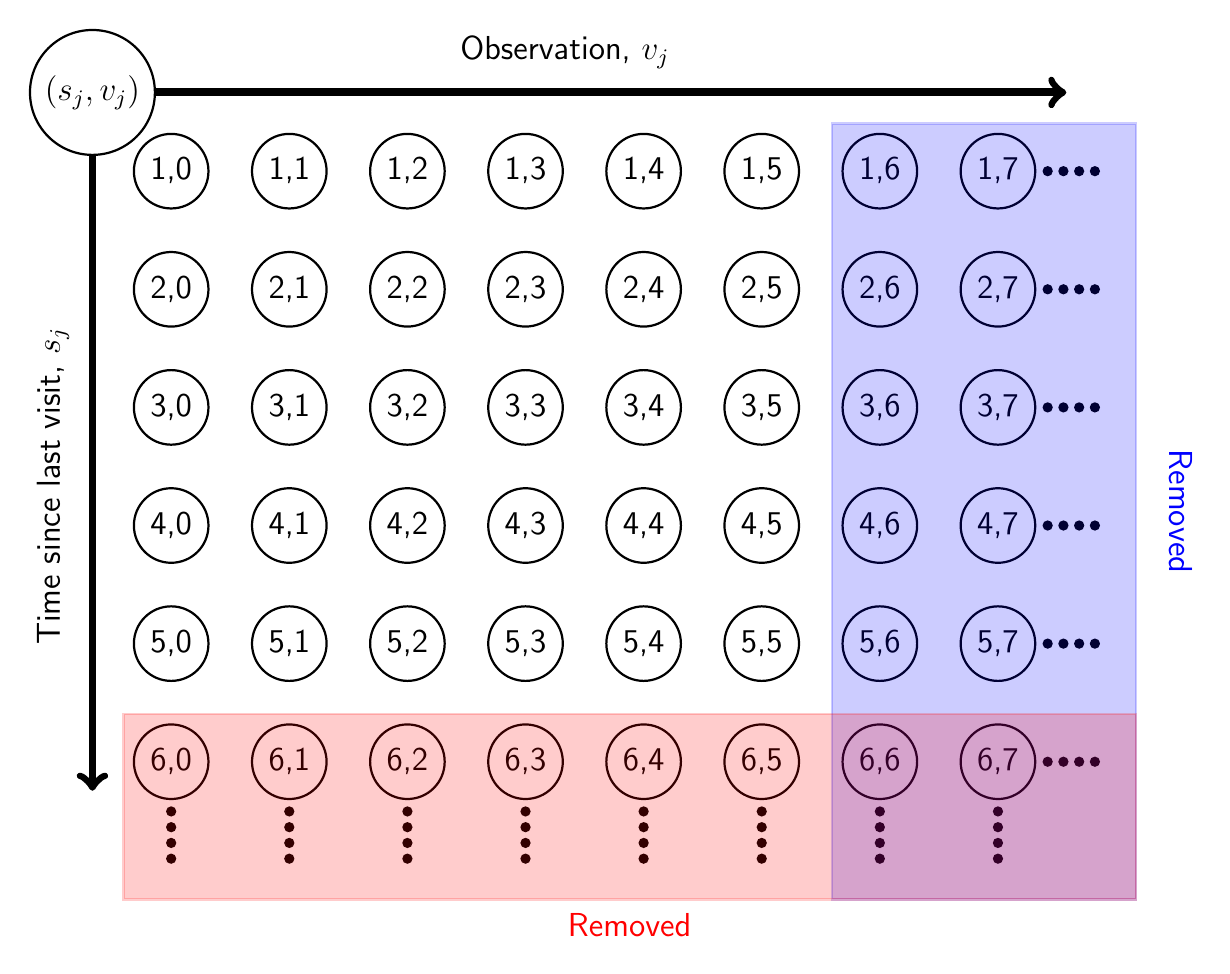
\begin{tikzpicture}[-,auto,node distance=1cm,
                    thick,main node/.style={circle,fill=white,draw,font=\sffamily\large,minimum size=0.5cm}]
 \foreach \x in {0,...,7}
    \foreach \y in {0,...,5} 
       {\pgfmathtruncatemacro{\label}{\x - 5 *  \y +21}
        \pgfmathtruncatemacro{\v}{\x}
        \pgfmathtruncatemacro{\s}{6-\y}
       \node [main node]  (\x\y) at (1.5*\x,1.5*\y) {\s,\v};} 

\node (XaxisLeft) [shift={(-0.5,1)}] at (05) {};
\node (XaxisRight) [shift={(1,1)}] at (75) {};

\node (YaxisBottom) [shift={(-1,-0.5)}] at (00) {};
\node (YaxisTop) [shift={(-1,1)}] at (05) {};

\draw[->,line width=1mm] (XaxisLeft)--(XaxisRight);
\draw[->,line width=1mm] (YaxisTop)--(YaxisBottom);

\node[font=\sffamily\large] (OLabel) [shift={(0.5,1.5)}] at (35) {Observation, $v_{j}$};
\node[font=\sffamily\large] (SLabel) [shift={(-1.5,0.5)}] at (02) {\rotatebox{90}{Time since last visit, $s_{j}$}};

\node[main node] (Example) [shift={(-1,1)}] at (05) {$(s_{j},v_{j})$};

\foreach \y in {0,...,5}
{\node (DottedStart\y) [shift={(0.5,0)}] at (7\y) {};
 \node (DottedEnd\y) [shift={(1.5,0)}] at (7\y) {};
 \draw[decorate sep={1mm}{2mm},fill] (DottedStart\y)--(DottedEnd\y);}
 
\foreach \x in {0,...,7}
{\node (\x DottedStart) [shift={(0,-0.5)}] at (\x0) {};
 \node (\x DottedEnd) [shift={(0,-1.5)}] at (\x0) {};
 \draw[decorate sep={1mm}{2mm},fill] (\x DottedStart)--(\x DottedEnd);
}

\node (Box1) [draw,thick,fit=(65) (60) (DottedEnd5) (DottedEnd0) (6DottedEnd) (7DottedEnd),fill,blue,opacity=0.2] {};

\node (Box2) [draw,thick,fit=(00) (70)(DottedEnd0) (0DottedEnd) (7DottedEnd),fill,red,opacity=0.2] {};

\node[font=\sffamily\large,color=blue] (Box1Text) [shift={(2.5,0)}] at (Box1) {\rotatebox{270}{Removed}};

\node[font=\sffamily\large,color=red] (Box2Text) [shift={(0,-1.5)}] at (Box2) {Removed};           

\end{tikzpicture}
}
\end{center}
\caption{State space diagram, with \textcolor{blue}{$b_{j}=5$} and \textcolor{red}{$B_{j}=4$} (e.g. $X_{j} \leq 3.7$)}
\end{myfigure}

\end{frame}

\begin{frame}{Markov Decision Process(MDP) formulation}
The available actions from any state is $\mathcal{A}(\bm{s})=\{j | A_{l(\bm{s}),j}=1 \}$. A transition from a state with a chosen action is $\phi(\bm{s},\bm{v},i)=(\widetilde{\bm{s}},\widetilde{\bm{v}})$ where $\widetilde{s}$ has; $\widetilde{s}_{i}=1$ and $\widetilde{s}_{j}=\min \{s_{j}+1,B_{j}+1 \} \forall j \neq i$ and $\widetilde{v}$ has; $\widetilde{v}_{i} \sim TPo(\lambda_{i},b_{i})$ and  $\widetilde{v}_{j}=v_{i} \forall j \neq i$.

Where $TPo(\lambda,b)$ is the Poisson distribution truncated at the value $b$. I.e
\begin{align*}
P(TPo(\lambda,b)=\begin{cases}
P(Po(\lambda) \text{ if } i \neq b \\
P(Po(\lambda) \geq i) \text{ if } i=b \\
0 \text{ Otherwise}
\end{cases}
\end{align*}

\end{frame}

\begin{frame}{Markov Decision Process(MDP) formulation}
The cost at a node is zero if that node is chosen, otherwise it is the cost of arrivals finishing in the next time period, plus the cost of local-observations finishing in the next time period.
\
$$C_{j}(\bm{s},\bm{v},i)=\begin{cases}
\begin{split}
&c_{j} \lambda_{j} \int_{s_{j}-1}^{s_{j}} P(X_{j} \leq t) dt \\
&+ c_{j}v_{j}P(s_{j}-1 < X_{j} \leq s_{j}) \text{ if } j \neq i 
\end{split} \\
0 \text{ if } j=i \\
\end{cases}$$.

Due to the finiteness of the state space, we can just focus on stationary, deterministic policies, $\pi: \Omega \rightarrow \mathcal{A}$ collected into $\Pi$, the set of stationary, deterministic policies.
\end{frame}

\begin{frame}{Markov Decision Process(MDP) formulation}
The patroller wants to choose a policy such that the long-run average cost is minimized. I.e. they want to find

\begin{align*}
C^{\text{OPT}}(\bm{s}_{0},\bm{v}_{0}) \equiv \min\limits_{\pi \in \Pi} \sum\limits_{i=1}^{n} V_{i}(\pi,\bm{s}_{0},\bm{v}_{0})
\end{align*}
where,
\begin{align*}
V_{i}(\pi,\bm{s}_{0},\bm{v}_{0}) \equiv \lim\limits_{N \rightarrow \infty} \frac{1}{N} \sum\limits_{k=0}^{N-1} C_{i}(\phi^{k}_{\pi}(\bm{s}_{0},\bm{v}_{0}),\pi(\phi^{k}_{\pi}(\bm{s}_{0},\bm{v}_{0})))
\end{align*}
Where $V_{i}(\pi,\bm{s}_{0},\bm{v}_{0})$ is the long-run average cost incurred at node $i$ under the policy, $pi$ and $\phi^{k}_{\pi}(\bm{s}_{0},\bm{v}_{0})$ is the state after $k$ transitions starting from $(\bm{s}_{0},\bm{v}_{0})$ under the policy $\pi$.

\end{frame}

\begin{frame}{Problem Relaxation: Multiple Node}
We now relax the problem to that of a patroller who can visit multiple nodes in the next timer period.

We will call this Problem the \textit{multiple node} (MN) problem. To extend ourselves to this problem we will create a new class of polices, $\Pi^{\text{MN}}$ which will allow the patroller to visit any set of nodes during the next time period.

\begin{align*}
\pi : \Omega \rightarrow \{\bm{\alpha} \, | \, \alpha_{i} \in \{0,1 \} \text{ for } i=1,...,n \}
\end{align*}

Where $\alpha_{i}=1$ if the patroller will visit node $i$ in the next time period and $\alpha_{i}=0$ if the patroller will not visit node $i$ in the next time period.
Note. $\Pi \subset \Pi^{\text{MN}}$.
\end{frame}

\begin{frame}{Total-rate constraint}
We now define the long-run rate at which the patroller visits node $i$, following $\pi$

\begin{align*}
\mu_{i}(\pi,\bm{s}_{0},\bm{v}_{0})=\lim\limits_{N \rightarrow \infty} \frac{1}{N} \sum\limits_{k=0}^{N-1} \alpha_{\psi_{\pi}^{k}(\bm{s}_{0},\bm{v}_{0}),i}
\end{align*}

We now impose the \textit{total-rate} constraint, that is the long-run overall visit rate to all nodes is no greater than 1. 

\begin{align*}
\sum\limits_{i=1}^{n} \mu_{i}(\pi,\bm{s}_{0},\bm{v}_{0}) \leq 1 \quad \forall (\bm{s}_{0},\bm{v}_{0}) \in \Omega
\end{align*}

and we denote the set of policies, which satisfy this constraint by $\Pi^{\text{TR}}$

Again $\Pi \subset \Pi^{\text{TR}}$ and we seek to find $C^{\text{TR}}$.
\end{frame}

\begin{frame}{Lagrangian relaxation}
We now relax the problem again by incorporating the total rate constraint into the objective function, with a Lagrange multiplier, $\omega \geq 0$. This forms

\begin{align*}
C(\omega)&=\min_{\pi \in \Pi^{\text{MN}}} \left\{ \sum\limits_{i=1}^{n} V_{i}(\pi) + \omega \left( \sum\limits_{i=0}^{n} \mu_{i}(\pi) -1 \right) \right\} \\
&=\min_{\pi \in \Pi^{\text{MN}}} \sum\limits_{i=1}^{n} (V_{i}(\pi)+\omega \mu_{i}(\pi)) - \omega
\end{align*}

By incorporating the total-rate constraint as a Lagrange multiplier we can drop the constraint, so that the patroller can choose to visit any number of nodes in each time period (admittedly costing $\omega$).
\end{frame}

\begin{frame}{Linking reduced problems}
We have that for any $\omega \geq 0$

\begin{align*}
C^{\text{TR}}=\min_{\pi \in \Pi^{\text{TR}}} \sum\limits_{i=1}^{n} V_{i}(\pi) &\geq \min_{\pi \in \Pi^{\text{TR}}} \left\{ \sum\limits_{i=1}^{n} V_{i}(\pi) + \omega \left( \sum\limits_{i=0}^{n} \mu_{i}(\pi) -1 \right) \right\} \\
&\geq \min_{\pi \in \Pi^{\text{MN}}} \left\{ \sum\limits_{i=1}^{n} V_{i}(\pi) + \omega \left( \sum\limits_{i=0}^{n} \mu_{i}(\pi) -1 \right) \right\}=C(\omega)
\end{align*}

The first inequality follows as the total-rate constraint is obeyed in $\Pi^{\text{TR}}$ and hence the $\omega \left( \sum\limits_{i=0}^{n} \mu_{i}(\pi) -1 \right) \leq 0$ and the second holds, as the total rate constraint is dropped and we have got a bigger state space, so we can only do better and hence possibly get a lower value.

Hence we have a string of inequalities $C^{\text{OPT}} \geq C^{\text{TR}} \geq C(\omega)$.
\end{frame}

\begin{frame}{Single node problem}
We now want to find $C(\omega)=\min_{\pi \in \Pi^{\text{MN}}} \sum\limits_{i=1}^{n} (V_{i}(\pi)+\omega \mu_{i}(\pi)) - \omega$ and we can split this problem up to just solve at each node.

That is consider a every node, $i$, try to minimize $V_{i}(\pi)+\omega \mu_{i}(\pi)$, where $\omega$ can be interpreted as the service charge for visiting.

For now we drop the node subscript and just try to find the following

\begin{align*}
\min_{\pi \in \Pi^{\text{MN}}} V(\pi) + \omega \mu(\pi)
\end{align*}

\end{frame}

\begin{frame}{Deterministic attack times}
Before looking at solving the single node problem, we will assume the attack times are deterministic, to make the cost function easier to handle.

When we use $X_{j}=x_{j}$ we get a cost function of.

For $s_{j} < B_{j}$
\begin{align*}
C_{j}(\bm{s},\bm{v},i)=0
\end{align*}

For $s_{j}=B_{j}$
\begin{align*}
C_{j}(\bm{s},\bm{v},i)= \begin{cases}
c_{j} \lambda_{j} R_{j} + c_{j} v_{j}  \text{ for } i \neq j \\
0 \text{ for } i=j \\
\end{cases}  
\end{align*}

For $s_{j}=B_{j}+1$
\begin{align*}
C_{j}(\bm{s},\bm{v},i)= \begin{cases}
c_{j} \lambda_{j} \text{ for } i \neq j \\
0 \text{ for } i=j \\
\end{cases}
\end{align*}

\end{frame}

\end{document}